\subsection{VehiclesHubDatabase}
The \verb|VehiclesHubDatabase| played a key role in this project. Coming to the realization on \hyperref[phase3]{\ref{phase3} Phase 3 - Signal R} the project needed a database that could handle the continuous changes in each \verb|Vehicle| position in real time. During research the group was unable to conclude on any databases that would fit our requirement. Hence, \verb|VehiclesHubDatanbase| was created to serve as a live in-memory database that could continuously update the positions of each vehicle on each lane.
\begin{figure}[h!]
	\centering
	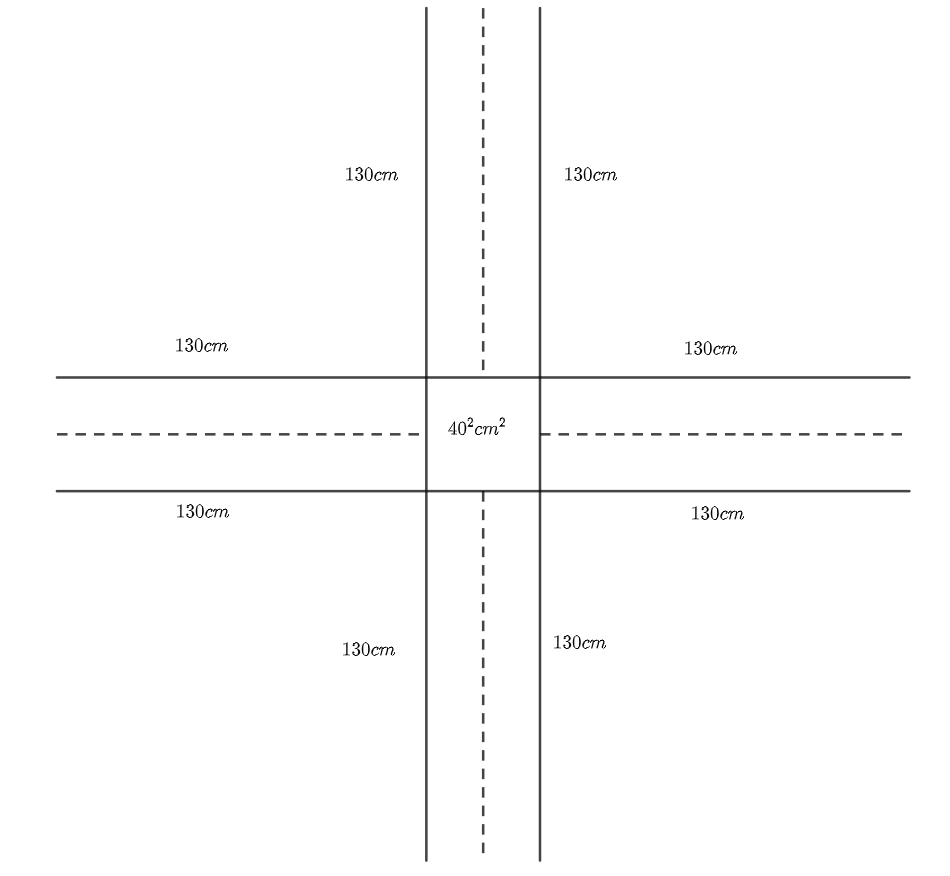
\includegraphics[width=1\linewidth]{figures/intersection_concept}
	\caption{This figure shows two roads each with two lanes and a total length of 300cm. The overlapping part forms a square which is the intersection. This configuration was heavily considered when creating representational models on the server, and also used for the demo as a result.}
	\label{fig:intersectionconcept}
\end{figure}

Before starting with \verb|VehiclesHubDatabase|, it was required to define what a road, lane and intersection is, respectively. Thus, \verb|Road.cs|, \verb|Lane.cs| and \verb|Intersection.cs| was developed. Consequently, \verb|VehiclesHubDatabase| was created.
\begin{csharp}
public class VehiclesHubDatabase : IVehiclesHubDatabase
{
	private readonly Intersection _intersection;
	
	private readonly HashSet<Vehicle> _vehicles = new();
	private readonly HashSet<Lane> _lanes = new();
	public int Count => _vehicles.Count;
	private readonly Dictionary<string, Vehicle> _connectionIds = new();
	private readonly Dictionary<Vehicle, string> _vehiclesConnectionId = new();
	...
	public double SpeedLimit => 80;
	...
}
\end{csharp}

Currently, \verb|VehiclesHubDatabase| only holds one intersection, due to time constraint this was not extended for a configuration with multiple intersections. Moreover, both vehicles and lanes are stored inside a hashset for fast retrieval. In addition, \verb|Count| is used in \verb|WaitForVehicles|, elaborated in sub-section \hyperref[handshake]{\ref{handshake} Handshake and listener}, and \verb|_connectionId| and \verb|_vehiclesConnectionId| is used during \verb|Patch| to invoke \verb|adjust_velocity| on individual vehicles. While, \verb|SpeedLimit| defines the upper speed vehicles are limited to on the two roads shown in \hyperref[fig:intersectionconcept]{Figure \ref{fig:intersectionconcept}}.

The road configuration found in \hyperref[fig:intersectionconcept]{Figure \ref{fig:intersectionconcept}} is defined in the constructor using a builder pattern.
\begin{csharp}
public class VehiclesHubDatabase : IVehiclesHubDatabase
{
	...
	public VehiclesHubDatabase()
	{
		_intersection = new Intersection().
			AddRoad(new Road {Length = 300}.
				AddLane(null, true).
				AddLane()).
		AddRoad(new Road {Length = 300}.
				AddLane(null, true).
				AddLane());
		
		_intersection.ConnectedLanes().
			ForEach(lane => _lanes.Add(lane));
	}
	...
}
\end{csharp}

Lastly, \verb|VehiclesHubDatabase| is added as a singleton service in \verb|Program.cs| to ensure that we have a static database throughout the lifetime of the program:
\begin{csharp}
...
builder.Services.AddSingleton<IVehiclesHubDatabase>(new VehiclesHubDatabase());
...
\end{csharp}

It is also worth to mention some of the core  functionalities of \verb|VehiclesHubDatabase|:

\subsubsection{Adding vehicles}
Calling the \verb|Add| method makes it possible to add vehicles:
\begin{csharp}
public class VehiclesHubDatabase : IVehiclesHubDatabase
{
	...
	public void Add(Vehicle vehicle, string? connectionId = null) {...}
	
	public void Add(Vehicle vehicle, Lane? lane = null) {...}
	...
}
\end{csharp}

\subsubsection{Removing vehicles}
Removing vehicles can be achieved by calling the \verb|Remove| method:
\begin{csharp}
public class VehiclesHubDatabase : IVehiclesHubDatabase
{
	...
	public void Remove(Vehicle vehicle) {...}
	...
}
\end{csharp}

\subsubsection{Updating vehicles}
Updating either a specific information of a vehicle or all vehicles can be done by calling the \verb|Update| method:
\begin{csharp}
public class VehiclesHubDatabase : IVehiclesHubDatabase
{
	...
	public void Update(Vehicle? vehicle = null) {...}
	...
}
\end{csharp}

\subsubsection{Fetching vehicles}
One can fetch an existing vehicle from the database by passing a vehicle with the same GUID with:
\begin{csharp}
public class VehiclesHubDatabase : IVehiclesHubDatabase
{
	...
	public Vehicle? Fetch(Vehicle vehicle) {...}
	...
}
\end{csharp}

\subsubsection{Get the connection Id of a particular vehicle}
By passing a vehicle into
\begin{csharp}
public class VehiclesHubDatabase : IVehiclesHubDatabase
{
	...
	public string? ConnectionId(Vehicle vehicle) {...}
	...
}
\end{csharp}
one can retrieve the connection Id that the given vehicle is using.

\subsubsection{Find vehicles approaching the intersection}
Maybe the most important feature of \verb|VehiclesHubDatabase| is the two method shown below:
\begin{csharp}
public class VehiclesHubDatabase : IVehiclesHubDatabase
{
	...
	public IEnumerable<Vehicle> NextVehiclesIn() {...}
	public IEnumerable<Vehicle> OnlyFirstIntoNextVehiclesIn() {...}
}
\end{csharp}
The first method \verb|NextVehiclesIn| returns a list of vehicles currently approaching the intersection defined in the constructor, ordered with respect to the vehicle closest to the intersection. The latter method \verb|OnlyFirstIntoNextVehiclesIn| returns an ordered list of the closest vehicle per lane.